\documentclass[11pt]{article}

\usepackage[margin=1in]{geometry}
\usepackage[T1]{fontenc}
\usepackage{lmodern}
\usepackage{microtype}
\usepackage{graphicx}
\usepackage{booktabs}
\usepackage{array}
\usepackage{enumitem}
\usepackage{hyperref}
\usepackage{xcolor}
\usepackage{tikz}
\usepackage{pgfplots}
\usepackage{amsmath}
\usepackage{parskip}
\usepackage{tabularx}
\usepackage{float}
\usepackage{caption}
\usepackage{titlesec}

\usetikzlibrary{arrows.meta,positioning,shapes.geometric,calc}
\pgfplotsset{compat=1.18}
\hypersetup{
    colorlinks=true,
    linkcolor=blue!55!black,
    urlcolor=blue!55!black,
    citecolor=blue!55!black,
    pdftitle={From Deepfake Detector to AI Shield - Part I},
    pdfauthor={Abdelrahman Mohamed}
}

\definecolor{navy}{HTML}{123B5D}
\definecolor{gold}{HTML}{C28C2D}
\definecolor{softblue}{HTML}{EAF2F8}
\definecolor{softgray}{HTML}{F5F6F8}
\definecolor{softgreen}{HTML}{EAF7EE}
\definecolor{softred}{HTML}{FCEEEE}
\definecolor{softyellow}{HTML}{FFF8E7}

\titleformat{\section}{\Large\bfseries\color{navy}}{}{0em}{}
\titleformat{\subsection}{\large\bfseries\color{navy}}{}{0em}{}
\setcounter{tocdepth}{2}
\captionsetup{font=small,labelfont=bf}

\newcommand{\callout}[2]{%
\begin{center}
\fcolorbox{navy}{softgray}{%
\parbox{0.94\linewidth}{%
\raggedright
\textbf{#1}\par
\vspace{0.35em}
#2
}}
\end{center}
}

\newcommand{\summarycard}[3]{%
\fcolorbox{navy}{#1}{%
\parbox[c][3.4cm][t]{0.94\linewidth}{%
\raggedright
\textbf{#2}\par\vspace{0.35em}
\small #3
}}
}

\newcommand{\metriccard}[3]{%
\fcolorbox{navy}{#1}{%
\parbox[c][2.2cm][c]{0.92\linewidth}{%
\centering
\textbf{#2}\par
\vspace{0.25em}
{\Large\bfseries #3}
}}
}

\begin{document}

\begin{titlepage}
    \centering
    \vspace*{1.0cm}
    {\large\color{navy}\textbf{Mini-Capstone Report}\par}
    \vspace{0.45cm}
    {\Huge\bfseries\color{navy} From Deepfake Detector to AI Shield\par}
    \vspace{0.3cm}
    {\Large Part I: Executive Summary and Academic Abstract\par}
    \vspace{0.8cm}
    {\large Abdelrahman Mohamed\par}
    \vspace{0.2cm}
    {\normalsize April 2026\par}

    \vspace{1.0cm}
    \fcolorbox{navy}{softblue}{%
    \parbox{0.88\linewidth}{%
    \centering
    \textbf{Project focus.} My broader capstone goal is a detector for AI-generated and AI-manipulated media. This part presents the first completed image-focused detector, the hard cases that exposed its limits, and the redesigned four-phase image pipeline that will later extend to video.
    }}

    \vspace{1.0cm}
    \begin{center}
    \begin{minipage}[t]{0.29\textwidth}
    \centering
    \metriccard{softblue}{Validation Accuracy}{0.9651}
    \end{minipage}\hfill
    \begin{minipage}[t]{0.29\textwidth}
    \centering
    \metriccard{softgreen}{Validation Precision}{0.9919}
    \end{minipage}\hfill
    \begin{minipage}[t]{0.29\textwidth}
    \centering
    \metriccard{softred}{Test Accuracy}{0.8577}
    \end{minipage}
    \end{center}

    \vspace{0.9cm}
    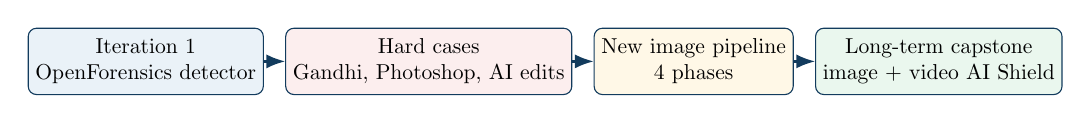
\begin{tikzpicture}[
        scale=0.78,
        transform shape,
        node distance=0.55cm and 0.35cm,
        box/.style={draw=navy, rounded corners=3pt, minimum width=2.55cm, minimum height=1.08cm, align=center},
        arrow/.style={-{Latex[length=2.4mm]}, thick, draw=navy}
    ]
    \node[box, fill=softblue] (a) {Iteration 1\\OpenForensics detector};
    \node[box, right=of a, fill=softred] (b) {Hard cases\\Gandhi, Photoshop, AI edits};
    \node[box, right=of b, fill=softyellow] (c) {New image pipeline\\4 phases};
    \node[box, right=of c, fill=softgreen] (d) {Long-term capstone\\image + video AI Shield};
    \draw[arrow] (a) -- (b);
    \draw[arrow] (b) -- (c);
    \draw[arrow] (c) -- (d);
    \end{tikzpicture}

    \vfill
    \fcolorbox{navy}{softgray}{%
    \parbox{0.86\linewidth}{%
    \centering
    \textbf{Document contents.} This file contains a one-page executive summary for a general audience and a technical abstract for readers with more ML background.
    }}
\end{titlepage}

\pagenumbering{roman}
\thispagestyle{empty}
\tableofcontents
\clearpage
\pagenumbering{arabic}

\section*{Part 1: Executive Summary and Academic Abstract}
\addcontentsline{toc}{section}{Part 1: Executive Summary and Academic Abstract}

\subsection*{Executive Summary}
\addcontentsline{toc}{subsection}{Executive Summary}

\noindent\textbf{One-sentence takeaway.} I built a real deepfake detector that worked well on a benchmark of real and fake \emph{face images}, but hard cases showed me that this first detector covered only one part of the bigger authenticity problem.

\vspace{0.45em}

\begin{center}
\begin{minipage}[t]{0.345\textwidth}
\centering
\summarycard{softblue}{What I already built}{
I trained, compared, and deployed a working image-level detector on the OpenForensics benchmark. The strongest preserved model was \textbf{EfficientNetV2-B0}, selected after comparing several CNN candidates and shipped as a usable app.
}
\end{minipage}\hfill
\begin{minipage}[t]{0.33\textwidth}
\centering
\summarycard{softred}{What changed the project}{
The turning point was a pattern of hard cases: Gandhi taking a selfie, Photoshop-style portrait edits, and AI-edited people images that looked plausible enough to expose the difference between realism and authenticity.
}
\end{minipage}\hfill
\begin{minipage}[t]{0.32\textwidth}
\centering
\summarycard{softgreen}{What comes next}{
My next iteration is an \textbf{AI Shield}: a four-phase system that starts with image evidence and later extends to video. I have already started the first new-pipeline pilot on Tiny-GenImage in Google Colab.
}
\end{minipage}
\end{center}

My larger capstone goal is to build a detector for \textbf{AI-generated and AI-manipulated images and videos}. I started with images first because that was the most practical way to build one strong layer, deploy it, and learn from its limits before adding video and more complex evidence.

The first detector itself was meaningful. The best preserved model was an \textbf{EfficientNetV2-B0} classifier trained on OpenForensics. In the saved experiment artifacts, it reached \textbf{0.9651 validation accuracy}, \textbf{0.9919 validation precision}, and \textbf{0.9824 validation AUC}. On a harder held-out test set, the score dropped to \textbf{0.8577 accuracy}. That already suggested that benchmark success does not automatically mean a detector is trustworthy once the conditions become messier.

But OpenForensics mainly gave me \textbf{real and fake face images}. That was a strong place to start, because it let me build a serious first image detector. At the same time, it did \textbf{not} cover the full pipeline I ultimately care about: broader AI-generated images, Photoshop-style edits outside narrow face-forgery settings, AI-edited photographs, claim-based authenticity, provenance, and later video. That gap is one of the main reasons the project changed.

\begin{center}
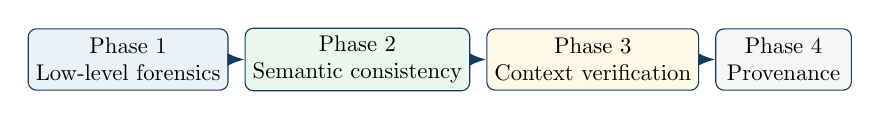
\begin{tikzpicture}[
    scale=0.82,
    transform shape,
    node distance=0.5cm and 0.25cm,
    box/.style={draw=navy, rounded corners=3pt, minimum width=2.1cm, minimum height=0.95cm, align=center},
    arrow/.style={-{Latex[length=2.2mm]}, thick, draw=navy}
]
\node[box, fill=softblue] (f1) {Phase 1\\Low-level forensics};
\node[box, right=of f1, fill=softgreen] (f2) {Phase 2\\Semantic consistency};
\node[box, right=of f2, fill=softyellow] (f3) {Phase 3\\Context verification};
\node[box, right=of f3, fill=softgray] (f4) {Phase 4\\Provenance};
\draw[arrow] (f1) -- (f2);
\draw[arrow] (f2) -- (f3);
\draw[arrow] (f3) -- (f4);
\end{tikzpicture}

\small\textbf{Figure 1.} The redesigned image pipeline now has four explicit phases. The current work already completed the first detector and started the new phase-1 pilot.
\end{center}

So the new pipeline is more explicit than the first one. It begins with \textbf{low-level forensics}, which asks whether the image carries generation or manipulation traces. Then it adds \textbf{semantic consistency}, which asks whether suspicious regions such as hands, reflections, and boundaries make sense together. After that come \textbf{context verification}, which asks whether the content fits the claim being made about it, and \textbf{provenance}, which asks whether the file has any trustworthy source history. Once this image pipeline is stable, the longer-term capstone extends the same logic to video.

To support that broader direction, the data also had to change. The first detector depended mostly on OpenForensics, which was useful for face-focused real/fake classification. The new pipeline needs broader image coverage as well. That is why I started a new pilot on \textbf{Tiny-GenImage} in Google Colab. Tiny-GenImage gives a much wider range of real and AI-generated images than the first face-only benchmark, so it is a better first step for the redesigned phase-1 image pipeline. After that, I plan to bring in edited-image benchmarks and later video datasets so the system can gradually cover more realistic cases instead of staying inside a narrow benchmark setting.

\begin{table}[H]
\centering
\small
\begin{tabularx}{0.98\textwidth}{>{\raggedright\arraybackslash}p{2.8cm} >{\raggedright\arraybackslash}p{3.4cm} >{\raggedright\arraybackslash}X}
\toprule
\textbf{Main data source} & \textbf{What it covers} & \textbf{Why it matters} \\
\midrule
OpenForensics & Real/fake face images and face-manipulation cases & Strong first benchmark for the first detector, but too narrow to represent the full capstone pipeline by itself. \\
Tiny-GenImage & Broader real vs AI-generated images & First practical pilot for the redesigned phase-1 image pipeline in Colab. \\
Later edited-image and video benchmarks & Photoshop-style edits, AI-edited images, and video-specific cases & Needed to move from a narrow image benchmark toward a broader authenticity system. \\
\bottomrule
\end{tabularx}
\caption{Why the project needed new data as well as a new pipeline.}
\end{table}

\callout{Why this matters for a general audience}{
The real value of the project is not only that I trained a detector. The value is that I built one, deployed it, tested it on hard cases, saw exactly where it stopped being enough, and used that evidence to design a stronger long-term AI Shield.
}

\noindent\textbf{What I want someone to remember after one page:}
\begin{enumerate}[leftmargin=1.5em]
    \item I already built a real deepfake detector and tested it seriously.
    \item That first detector was based mainly on real and fake face images, so it was a strong first step but not the full capstone pipeline.
    \item Hard cases, including Gandhi, Photoshop-style edits, and AI-edited portraits, showed me why the project needed both broader data and a new four-phase design.
    \item I have already started the first model of the redesigned image pipeline in Google Colab on Tiny-GenImage, and the long-term goal remains an image-and-video AI Shield.
\end{enumerate}

\clearpage
\subsection*{Academic Abstract}
\addcontentsline{toc}{subsection}{Academic Abstract}

This mini-capstone documents the first completed iteration of a broader capstone whose long-term goal is an AI-generated media detector for both \textbf{images and video}. I began with the image branch and built a deployable detector using OpenForensics and transfer learning with \textbf{EfficientNetV2-B0} \cite{le2021openforensics,tan2021efficientnetv2}. The preserved pipeline standardized RGB loading, resizing to \textbf{256$\times$256}, normalization, augmentation, and thresholded sigmoid-based inference. Across the saved model comparisons, EfficientNetV2-B0 was the strongest preserved baseline, achieving \textbf{0.9651 validation accuracy}, \textbf{0.9919 validation precision}, and \textbf{0.9824 validation AUC}; on a harder held-out test set, performance dropped to \textbf{0.8577 accuracy}, indicating sensitivity to distribution shift and post-processing.

A central lesson of this first iteration is that the original dataset and pipeline were too narrow for the broader authenticity problem. OpenForensics mainly provided real and fake face images, which made it a strong first benchmark but did not cover the wider range of AI-generated images, Photoshop-style edits, AI-edited photos, provenance signals, and video cases needed for the long-term capstone. This motivated a redesigned four-phase image pipeline: low-level forensic modeling, semantic consistency analysis, contextual claim verification, and provenance analysis. I have already started that redesign by training the first new-pipeline pilot in \textbf{Google Colab} on \textbf{Tiny-GenImage}, using a balanced subset of \textbf{4,000} training images and \textbf{1,000} validation images as a practical first run. The next methodological steps are a \textbf{variational autoencoder} for anomaly-sensitive forensic modeling \cite{kingma2014vae}, an \textbf{attention-based} semantic layer \cite{vaswani2017attention}, and later multimodal reasoning and video extension.

\section*{Selected References for Part I}
\addcontentsline{toc}{section}{Selected References for Part I}

\begin{thebibliography}{9}

\bibitem{le2021openforensics}
T.-N. Le, H. H. Nguyen, J. Yamagishi, and I. Echizen,
\emph{OpenForensics: Large-Scale Challenging Dataset for Multi-Face Forgery Detection and Segmentation In-The-Wild},
ICCV, 2021.

\bibitem{tan2021efficientnetv2}
M. Tan and Q. V. Le,
\emph{EfficientNetV2: Smaller Models and Faster Training},
ICML, 2021.

\bibitem{kingma2014vae}
D. P. Kingma and M. Welling,
\emph{Auto-Encoding Variational Bayes},
ICLR, 2014.

\bibitem{vaswani2017attention}
A. Vaswani et al.,
\emph{Attention Is All You Need},
NeurIPS, 2017.

\end{thebibliography}

\end{document}
